\documentclass[a4paper]{article}
\usepackage{latexsym}
\usepackage[a4paper]{geometry}
\usepackage{color}
\usepackage{listings}
\usepackage[pdftex]{graphicx}
\usepackage{subfig}

\definecolor{Blue}{rgb}{0,0,0.5}
\definecolor{Green}{rgb}{0,0.75,0.0}
\definecolor{LightGray}{rgb}{0.6,0.6,0.6}
\definecolor{DarkGray}{rgb}{0.3,0.3,0.3}
\newcommand\matlabstyle{\lstset{language=Matlab,
   keywords={function,uint8,uint16,uint32,double,break,case,catch,continue,else,elseif,end,for,global,if,otherwise,persistent,return,switch,try,while},
   basicstyle=\ttfamily\small,
   breaklines=true,
   keywordstyle=\bfseries\color{Blue},
   commentstyle=\itshape\color{LightGray},
   stringstyle=\color{Green},
   numbers=left,
   numberstyle=\tiny\color{DarkGray},
   stepnumber=1,
   numbersep=10pt,
   backgroundcolor=\color{white},
   tabsize=2,
   showspaces=false,
   showstringspaces=false,
   captionpos=b}}

%Boldface text for type writer font
\usepackage{bold-extra} %\DeclareFontShape{OT1}{cmtt}{bx}{n}{<5><6><7><8><9><10><10.95><12><14.4><17.28><20.74><24.88>cmttb10}{}

%Break words properly at the end of a line (which isn't sloppy...)
\sloppy

% New definition of square root:
% it renames \sqrt as \oldsqrt
\let\oldsqrt\sqrt
% it defines the new \sqrt in terms of the old one
\def\sqrt{\mathpalette\DHLhksqrt}
\def\DHLhksqrt#1#2{%
\setbox0=\hbox{$#1\oldsqrt{#2\,}$}\dimen0=\ht0
\advance\dimen0-0.2\ht0
\setbox2=\hbox{\vrule height\ht0 depth -\dimen0}%
{\box0\lower0.4pt\box2}}

%Use command \exercise for each exercise
\newcounter{exerciseCount}
\setcounter{exerciseCount}{0}
\newcommand{\exercise}[1]{\addtocounter{exerciseCount}{1} \noindent \medskip {\large \textsf{\textbf{Exercise \arabic{exerciseCount} \--- #1}}} \par}
\renewcommand{\theenumi}{\textsf{\textbf{\alph{enumi}}}}

%Use command \code for code snippets
\newcommand{\code}[1]{\textnormal{\texttt{#1}}}

% Python environment
\lstnewenvironment{matlab}[1][]
{
\matlabstyle
\lstset{#1}
}
{}

% Python for external files
\newcommand\matlabexternal[2][]{{
\matlabstyle
\lstinputlisting[#1]{#2}}}

% Python for inline
\newcommand\matlabinline[1]{{\matlabstyle\lstinline!#1!}}
\usepackage{amsmath, amssymb, graphics, setspace}



\title{\textsf{Image Processing \\ Lab 1}}
\author{Han Kruiger \and Maarten Terpstra (s2028980)}
\date{\today}

\begin{document}
\maketitle
%!TEX root = report.tex
\exercise{1D wavelet transforms}
\subsection{\texorpdfstring{1D \(J\)-scale DWT}{1D J-scale DWT}}


\subsection{\texorpdfstring{1D inverse \(J\)-scale DWT}{1D inverse J-scale DWT}}


\clearpage
\exercise{Enhancement}
\subsection*{a - IPlogenhance}
Sometimes it can be desirable to increase the intensity of low-intensity pixels without enhancing high-intensity pixels too much. A way to achieve this goal is by compressing the dynamic range of an image. By applying the log transform an image may become more insightful than when the dynamic range is too large. The log transformation is: \[
                                                                                               s = c\mbox{ }log(1+r)
                                                                                              \]
In this formula the value $r$ represents the value of the pixel the transformation is applied to. The value $c$ is a constant chosen by the user. The following Matlab code applies the log transformation to an image. 
\matlabexternal{IPlogenhance.m}
Here the type of \verb image  is a $y \times x$-matrix. The output image is also an $y \times x$-matrix with the transformation applied.

\subsection*{b - Enhancing a fractured spine}
In order to make sure the implementation is correct and the log transformation is useful the operation is applied to an image that could benefit from a compressed dynamic range. Figures~\ref{fig:withoutEnhancement} and~\ref{fig:withEnhancement} are both pictures of a fractured spine, but figure~\ref{fig:withEnhancement} has the log transform applied to it with $c = 1.75$.
\begin{figure}
 \centering
 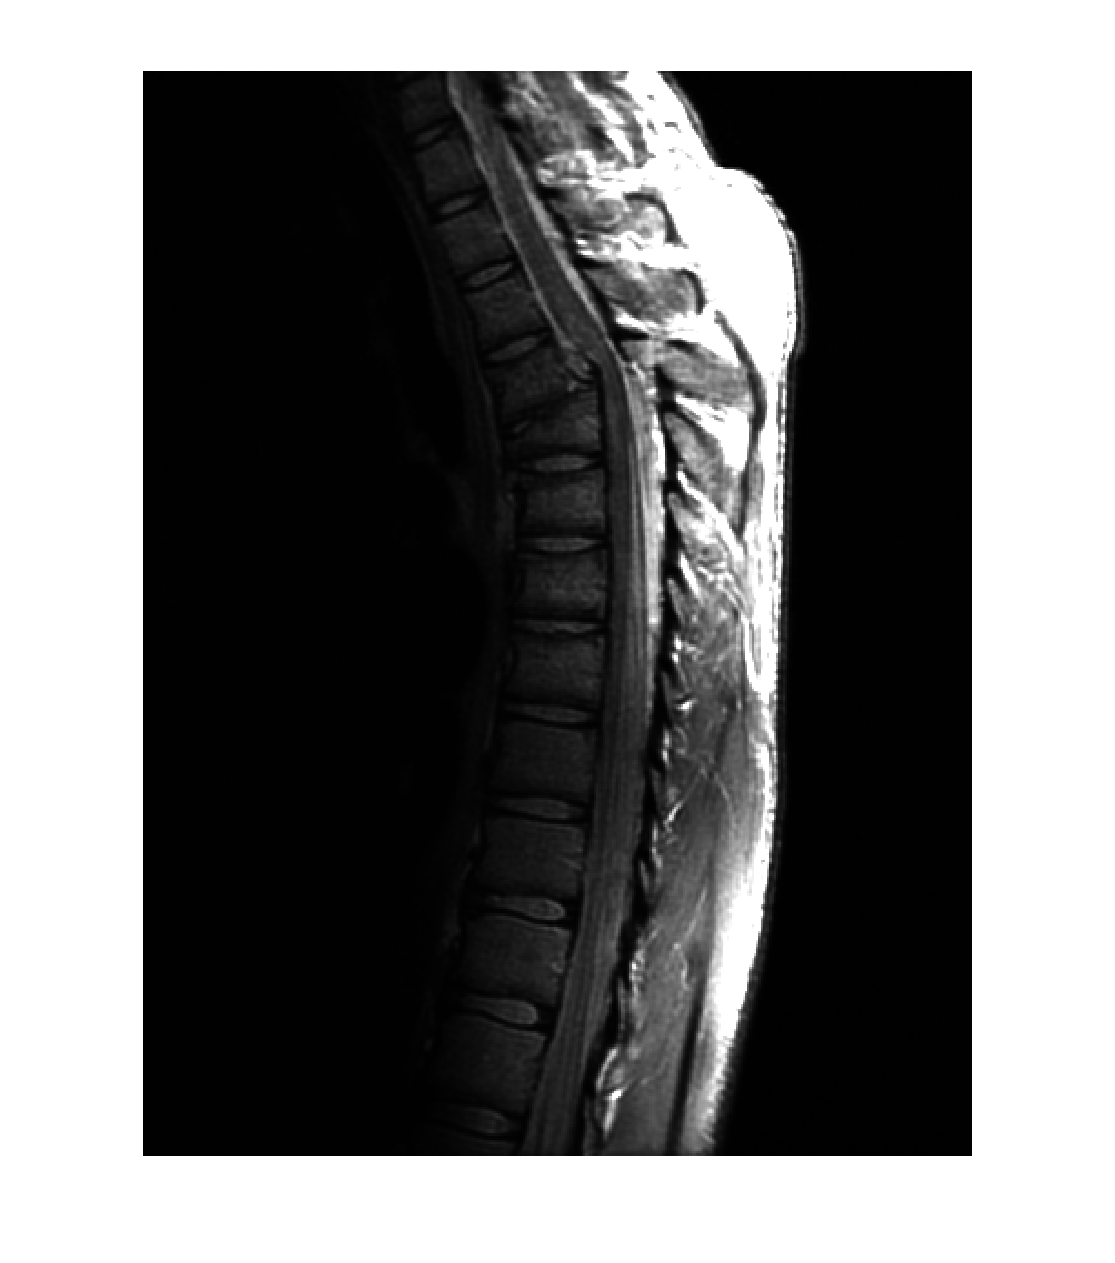
\includegraphics{breukLelijk.eps}
 \caption{An image of a fractured spine without enhancement applied}
 \label{fig:withoutEnhancement}
\end{figure}

\begin{figure}
 \centering
 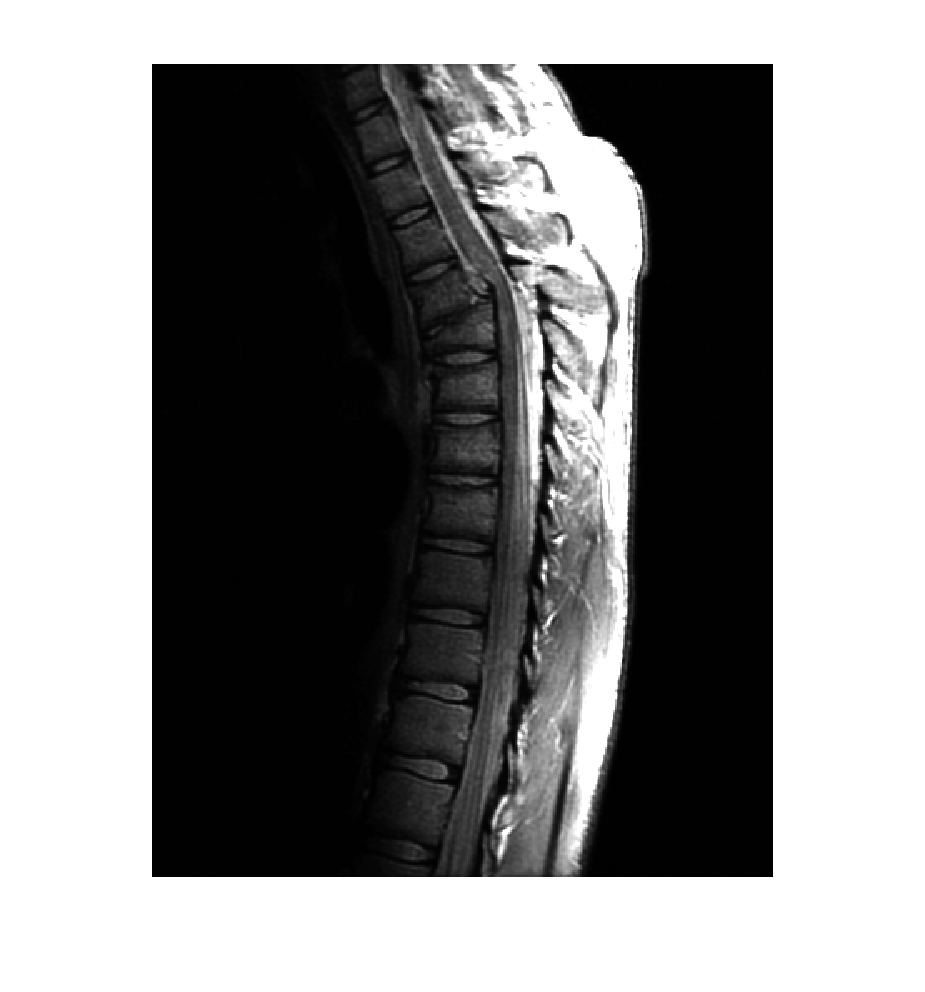
\includegraphics{breukMooi.eps}
 \caption{An image of a fractured spine with enhancement applied}
 \label{fig:withEnhancement}
\end{figure}

%!TEX root = report.tex
\exercise{Filtering}
\setcounter{subsection}{0}
\subsection{Gaussian lowpass filter}
We have implemented the Gaussian lowpass filter according to \cite[Equation~4.8-7]{gonzalez2002digital} in the function \texttt{IPgaussian\_lowpass} in the following function:
\matlabexternal{IPgaussian_lowpass.m}

For convenience, we've named the function \texttt{IPgaussian\_lowpass}, so it doesn't cause confusion with the highpass filter below.

The values \texttt{P} and \texttt{Q} are required as arguments, since the function has to compute the distance from the origin, which is in the center of the image.

\subsection{IPftfilter}
To filter frequencies from the frequency domain, we have written a function \texttt{IPftfilter} that performs filtering in the frequency domain.
The code that does this is listed below:
\matlabexternal{IPftfilter.m}

This function takes the following arguments:
\begin{itemize}
	\item \texttt{image}: The input image.
	\item \texttt{D\_0}: Cutoff frequency. This is the frequency that governs which region of the frequency domain will be `cut off'.
	\item \texttt{filter\_type}: The type of filter that is to be applied. Currently only the Gaussian lowpass filter (GLPF) and Gaussian highpass filter (GHPF) are implemented.
	\item \texttt{P} and \texttt{Q}: Dimensions of the Fourier domain that will be evaluated.
		If \texttt{P} or \texttt{Q} are higher than the original image, the image will be padded before being tranformed to the Fourier domain.
		After returning to the spatial domain, the redundant (padded) regions are sliced from the image prior to returning the filtered image.
		Setting \texttt{P} or \texttt{Q} lower than the original image is not advised, since parts of the image will be lost in that case.
\end{itemize}

The function transforms the image to the frequency domain, computes the filter, and subsequently multiplies the image with the filter, element-wise.
After transforming the image back to the spatial domain, taking the real part, and optionally doing some slicing, the filtered image is obtained.

\subsection{Lowpass characters}
Using the \texttt{IPftfilter} function on the image \texttt{characters.tif}, with the cutoff frequencies 5, 20, 30, 50 and 100, we've produced the images in Figure~\ref{fig:lowChars}.
We believe that with these values, the images in \cite[Figure~4.48]{gonzalez2002digital} are best approximated.
\begin{figure}[ht]
 \centering
 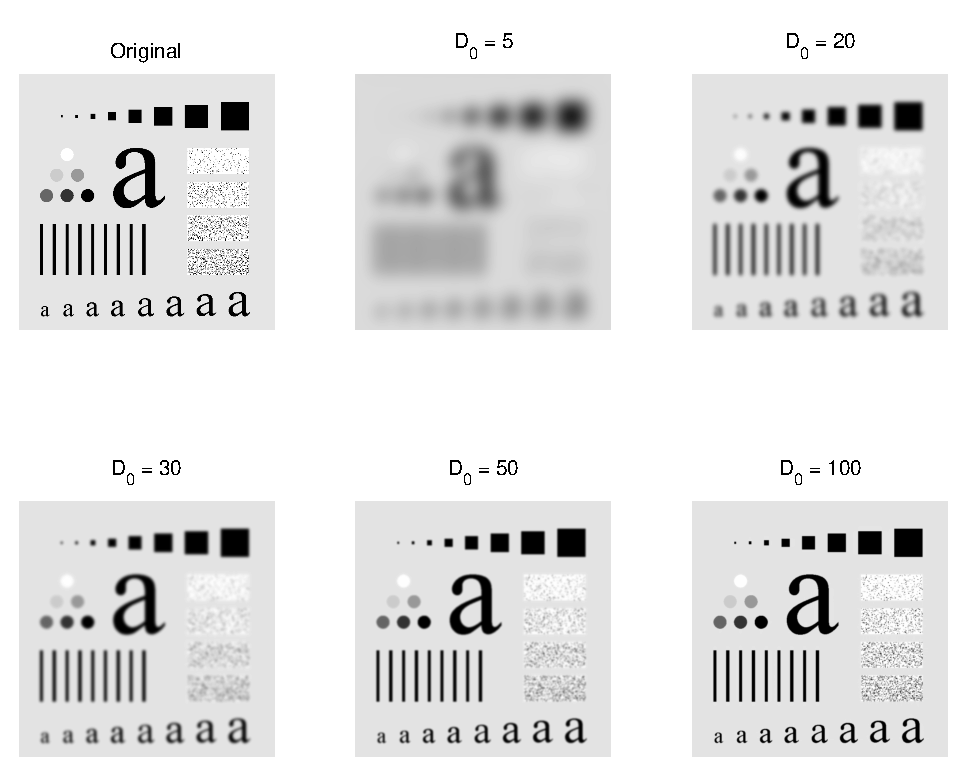
\includegraphics[width=\linewidth]{characters_low_pass.eps}
 \caption{
		The lowpass Gaussian filter at work for different cutoff frequencies.
		A higher cutoff frequency results in fewer details, since the region that is cut off is larger.
		A lower cutoff frequency results in a more blurred image, since the higher frequencies are cut off and only the low frequency signals persist.
	}
 \label{fig:lowChars}
\end{figure}

\clearpage

\subsection{Gaussian highpass filter}
The complementary Gaussian highpass filter was also implemented, as the function \texttt{IPgaussian\_highpass}.
Naturally, it was the inverse of the lowpass filter.
Because the highpass filter is very similar to the lowpass filter it doesn't need a detailed explanation, and is merely listed below:
\matlabexternal{IPgaussian_highpass.m}

\subsection{Highpass characters}
Using the same \texttt{IPftfilter} function, we've applief the highpass filter to the \texttt{characters} image.
To approximate \cite[Figure~4.56]{gonzalez2002digital}, the cutoff frequencies \(30\), \(60\) and \(100\) have been used. We have chosen these cutoff frequencies as they are mentioned in the caption of \cite[Figure~4.56]{gonzalez2002digital} and, as figure~\ref{fig:highChars} illustrate, the images seem very similar.
\begin{figure}[ht]
 \centering
 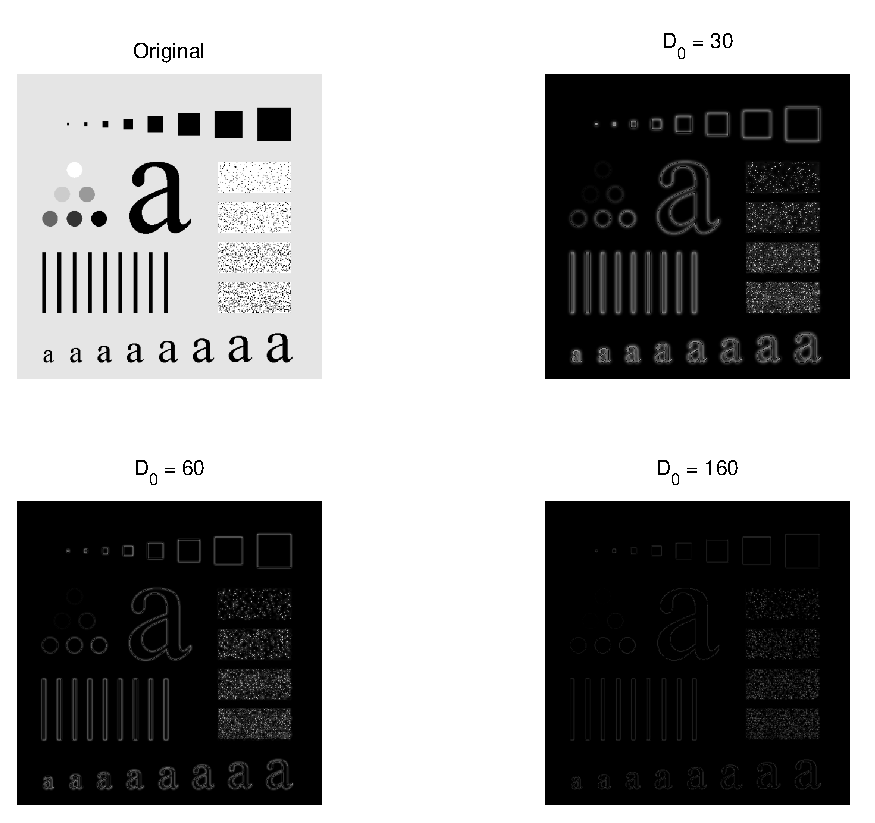
\includegraphics[width=\linewidth]{characters_high_pass.eps}
 \caption{
 	The highpass Gaussian filter at work for different cutoff frequencies.
 	Since higher frequencies persist when using a highpass filter, abrubt changes in the image (edges) appear clearly in the filtered image.
 	However, when the cutoff frequency is too high, too much information will be removed, resulting in an almost entirely black image.
 }
 \label{fig:highChars}
\end{figure}

\clearpage
% \begin{enumerate}
% \item
% Here comes an explanation how you can reduce the number of intensity levels of an image. After that, you also list the source code of the relevant function with some comments at each step.
% \lstinputlisting{IPcontrast.m}
% 
% \item
% \begin{center}
% \begin{tabular}{cccc}
%     \includegraphics[width=0.2\textwidth]{ctskull-256.png} &
%     \includegraphics[width=0.2\textwidth]{ctskull-256.png} &
%     \includegraphics[width=0.2\textwidth]{ctskull-256.png} &
%     \includegraphics[width=0.2\textwidth]{ctskull-256.png}\\
%     256 levels & 128 levels & 64 levels & 32 levels \\
%     \includegraphics[width=0.2\textwidth]{ctskull-256.png} &
%     \includegraphics[width=0.2\textwidth]{ctskull-256.png} &
%     \includegraphics[width=0.2\textwidth]{ctskull-256.png} &
%     \includegraphics[width=0.2\textwidth]{ctskull-256.png}\\
%     16 levels & 8 levels & 4 levels & 2 levels
% \end{tabular}
% \end{center}
% \end{enumerate}
% 
% 
% \exercise{Handing in}
% \noindent When you're done, construct an archive file (zip, tgz, or
% tar) which contains your report and Matlab files. Then hand it in
% according to the instructions of the lab assistants.

\end{document}
